


\begin{markdown}
#### List of Page Templates
Access to the list by opening the Organisation menu, then the Templates tab, and the Pages tab.
\end{markdown}

\begin{figure}[H]
    \centering
    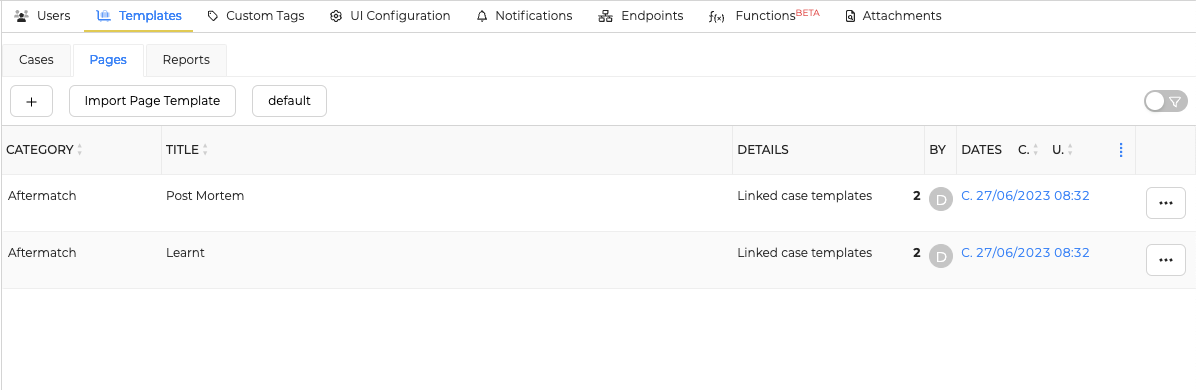
\includegraphics[width=\textwidth]{images/docs/org_admin/templates/page/organisation-pages-templates.png}
    \caption{List of pages templates}
    \label{fig:modules}
\end{figure}

\begin{markdown}

#### New Case template
Click the + button to create a new Page template.
\end{markdown}



\begin{figure}[H]
    \centering
    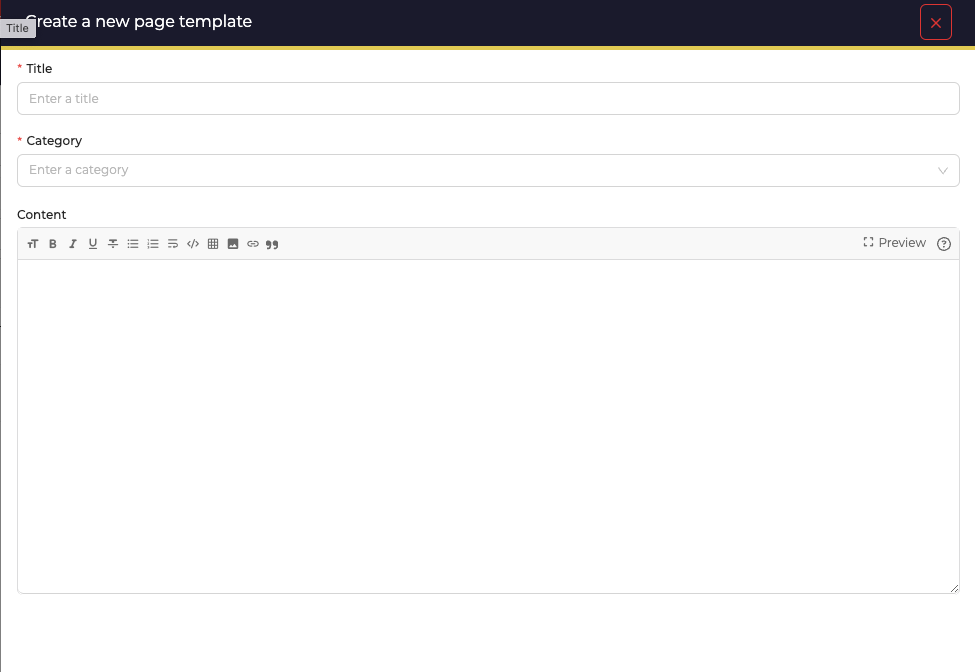
\includegraphics[width=\textwidth]{images/docs/org_admin/templates/page/organisation-pages-templates-2.png}
    \caption{New Page template}
    \label{fig:modules}
\end{figure}


Configuration parameters#
Title
Page template title. Used to identify the Page template with the API. Also used as a page title when the template is used in a case.
Category
Category for grouping pages on a common theme. Is used as a page tree in the case of.
Content
Default page content when the page template is used in a case.

